\documentclass[]{article}
\usepackage{lmodern}
\usepackage{amssymb,amsmath}
\usepackage{ifxetex,ifluatex}
\usepackage{fixltx2e} % provides \textsubscript
\ifnum 0\ifxetex 1\fi\ifluatex 1\fi=0 % if pdftex
  \usepackage[T1]{fontenc}
  \usepackage[utf8]{inputenc}
\else % if luatex or xelatex
  \ifxetex
    \usepackage{mathspec}
  \else
    \usepackage{fontspec}
  \fi
  \defaultfontfeatures{Ligatures=TeX,Scale=MatchLowercase}
\fi
% use upquote if available, for straight quotes in verbatim environments
\IfFileExists{upquote.sty}{\usepackage{upquote}}{}
% use microtype if available
\IfFileExists{microtype.sty}{%
\usepackage{microtype}
\UseMicrotypeSet[protrusion]{basicmath} % disable protrusion for tt fonts
}{}
\usepackage[margin=1in]{geometry}
\usepackage{hyperref}
\hypersetup{unicode=true,
            pdftitle={DATA 605 - Assignment 12},
            pdfauthor={Joshua Sturm},
            pdfborder={0 0 0},
            breaklinks=true}
\urlstyle{same}  % don't use monospace font for urls
\usepackage{graphicx,grffile}
\makeatletter
\def\maxwidth{\ifdim\Gin@nat@width>\linewidth\linewidth\else\Gin@nat@width\fi}
\def\maxheight{\ifdim\Gin@nat@height>\textheight\textheight\else\Gin@nat@height\fi}
\makeatother
% Scale images if necessary, so that they will not overflow the page
% margins by default, and it is still possible to overwrite the defaults
% using explicit options in \includegraphics[width, height, ...]{}
\setkeys{Gin}{width=\maxwidth,height=\maxheight,keepaspectratio}
\IfFileExists{parskip.sty}{%
\usepackage{parskip}
}{% else
\setlength{\parindent}{0pt}
\setlength{\parskip}{6pt plus 2pt minus 1pt}
}
\setlength{\emergencystretch}{3em}  % prevent overfull lines
\providecommand{\tightlist}{%
  \setlength{\itemsep}{0pt}\setlength{\parskip}{0pt}}
\setcounter{secnumdepth}{0}
% Redefines (sub)paragraphs to behave more like sections
\ifx\paragraph\undefined\else
\let\oldparagraph\paragraph
\renewcommand{\paragraph}[1]{\oldparagraph{#1}\mbox{}}
\fi
\ifx\subparagraph\undefined\else
\let\oldsubparagraph\subparagraph
\renewcommand{\subparagraph}[1]{\oldsubparagraph{#1}\mbox{}}
\fi

%%% Use protect on footnotes to avoid problems with footnotes in titles
\let\rmarkdownfootnote\footnote%
\def\footnote{\protect\rmarkdownfootnote}

%%% Change title format to be more compact
\usepackage{titling}

% Create subtitle command for use in maketitle
\newcommand{\subtitle}[1]{
  \posttitle{
    \begin{center}\large#1\end{center}
    }
}

\setlength{\droptitle}{-2em}
  \title{DATA 605 - Assignment 12}
  \pretitle{\vspace{\droptitle}\centering\huge}
  \posttitle{\par}
  \author{Joshua Sturm}
  \preauthor{\centering\large\emph}
  \postauthor{\par}
  \predate{\centering\large\emph}
  \postdate{\par}
  \date{April 29, 2018}

\usepackage{booktabs}
\usepackage{longtable}
\usepackage{array}
\usepackage{multirow}
\usepackage[table]{xcolor}
\usepackage{wrapfig}
\usepackage{float}
\usepackage{colortbl}
\usepackage{pdflscape}
\usepackage{tabu}
\usepackage{threeparttable}
\usepackage{threeparttablex}
\usepackage[normalem]{ulem}
\usepackage{makecell}

\begin{document}
\maketitle

\section{Objective}\label{objective}

\begin{itemize}
\item
  \begin{enumerate}
  \def\labelenumi{\arabic{enumi}.}
  \tightlist
  \item
    Provide a scatterplot of LifeExp\textasciitilde{}TotExp, and run
    simple linear regression. Do not transform the variables. Provide
    and interpret the F statistics, R\^{}2, standard error,and p-values
    only. Discuss whether the assumptions of simple linear regression
    met.
  \end{enumerate}
\item
  \begin{enumerate}
  \def\labelenumi{\arabic{enumi}.}
  \setcounter{enumi}{1}
  \tightlist
  \item
    Raise life expectancy to the 4.6 power (i.e., LifeExp\^{}4.6). Raise
    total expenditures to the 0.06 power (nearly a log transform,
    TotExp\^{}.06). Plot LifeExp\^{}4.6 as a function of TotExp\^{}.06,
    and r re-run the simple regression model using the transformed
    variables. Provide and interpret the F statistics, R\^{}2, standard
    error, and p-values. Which model is ``better?''
  \end{enumerate}
\item
  \begin{enumerate}
  \def\labelenumi{\arabic{enumi}.}
  \setcounter{enumi}{2}
  \tightlist
  \item
    Using the results from 3, forecast life expectancy when
    TotExp\^{}.06 =1.5. Then forecast life expectancy when
    TotExp\^{}.06=2.5.
  \end{enumerate}
\item
  \begin{enumerate}
  \def\labelenumi{\arabic{enumi}.}
  \setcounter{enumi}{3}
  \tightlist
  \item
    Build the following multiple regression model and interpret the F
    Statistics, R\^{}2, standard error, and p-values. How good is the
    model?\\
    LifeExp = b0+b1 x PropMd + b2 x TotExp +b3 x PropMD x TotExp
  \end{enumerate}
\item
  \begin{enumerate}
  \def\labelenumi{\arabic{enumi}.}
  \setcounter{enumi}{4}
  \tightlist
  \item
    Forecast LifeExp when PropMD=.03 and TotExp = 14. Does this forecast
    seem realistic? Why or why not?
  \end{enumerate}
\end{itemize}

\section{Import dataset}\label{import-dataset}

\subsection{Data Dictionary}\label{data-dictionary}

\begin{table}[H]
\centering\rowcolors{2}{gray!6}{white}

\resizebox{\linewidth}{!}{\begin{tabular}{ll}
\hiderowcolors
\toprule
Variable Name & Definition\\
\midrule
\showrowcolors
Country & Name of the country\\
LifeExp & Average life expectancy for the country in years\\
InfantSurvival & Proportion of those surviving to one year or more\\
Under5Survival & Proportion of those surviving to five years or more\\
TBFree & Proportion of the population without TB\\
\addlinespace
PropMD & Proportion of the population who are MDs\\
PropRN & Proportion of the population who are RNs\\
PersExp & Mean personal expenditures on healthcare in US dollars at average exchange rate\\
GovtExp & Mean government expenditures per capita on healthcare, US dollars at average exchange rate\\
TotExp & Sum of personal and government expenditures\\
\bottomrule
\end{tabular}}
\rowcolors{2}{white}{white}
\end{table}

\subsection{Data Structure}\label{data-structure}

\begin{table}[H]
\centering\rowcolors{2}{gray!6}{white}

\resizebox{\linewidth}{!}{\begin{tabular}{lrrrrrrrrrrrrr}
\hiderowcolors
\toprule
  & vars & n & mean & sd & median & trimmed & mad & min & max & range & skew & kurtosis & se\\
\midrule
\showrowcolors
Country* & 1 & 190 & 9.550000e+01 & 5.499242e+01 & 9.55000e+01 & 9.550000e+01 & 70.4235000 & 1.00e+00 & 1.90000e+02 & 1.89000e+02 & 0.0000000 & -1.2189633 & 3.9895697\\
LifeExp & 2 & 190 & 6.737895e+01 & 1.084785e+01 & 7.00000e+01 & 6.847368e+01 & 10.3782000 & 4.00e+01 & 8.30000e+01 & 4.30000e+01 & -0.7973539 & -0.2456855 & 0.7869854\\
InfantSurvival & 3 & 190 & 9.624474e-01 & 3.817270e-02 & 9.78500e-01 & 9.689276e-01 & 0.0244629 & 8.35e-01 & 9.98000e-01 & 1.63000e-01 & -1.3392518 & 1.1070308 & 0.0027693\\
Under5Survival & 4 & 190 & 9.459421e-01 & 6.288300e-02 & 9.74500e-01 & 9.584079e-01 & 0.0289107 & 7.31e-01 & 9.97000e-01 & 2.66000e-01 & -1.5708451 & 1.7147500 & 0.0045620\\
TBFree & 5 & 190 & 9.980375e-01 & 2.450900e-03 & 9.99215e-01 & 9.984857e-01 & 0.0010156 & 9.87e-01 & 9.99980e-01 & 1.29800e-02 & -1.6601038 & 2.6962678 & 0.0001778\\
\addlinespace
PropMD & 6 & 190 & 1.795400e-03 & 3.627600e-03 & 1.04740e-03 & 1.308700e-03 & 0.0013654 & 1.96e-05 & 3.51290e-02 & 3.51094e-02 & 7.5169037 & 64.2463055 & 0.0002632\\
PropRN & 7 & 190 & 4.133600e-03 & 6.060400e-03 & 2.75840e-03 & 3.259200e-03 & 0.0030487 & 8.83e-05 & 7.08387e-02 & 7.07504e-02 & 7.2505578 & 74.8125351 & 0.0004397\\
PersExp & 8 & 190 & 7.420000e+02 & 1.353999e+03 & 1.99500e+02 & 3.866974e+02 & 256.4898000 & 3.00e+00 & 6.35000e+03 & 6.34700e+03 & 2.4790093 & 5.6380247 & 98.2294089\\
GovtExp & 9 & 190 & 4.095349e+04 & 8.614065e+04 & 5.38500e+03 & 1.767133e+04 & 7692.4701000 & 1.00e+01 & 4.76420e+05 & 4.76410e+05 & 2.8602374 & 8.3912307 & 6249.2993052\\
TotExp & 10 & 190 & 4.169549e+04 & 8.744985e+04 & 5.54100e+03 & 1.806003e+04 & 7899.2928000 & 1.30e+01 & 4.82750e+05 & 4.82737e+05 & 2.8511964 & 8.3228612 & 6344.2791865\\
\bottomrule
\end{tabular}}
\rowcolors{2}{white}{white}
\end{table}

The dataset has 9 predictor variables, and 190 cases. Each case
represents a country in the world, with different statistics about their
quality of healthcare.

\section{1.}\label{section}

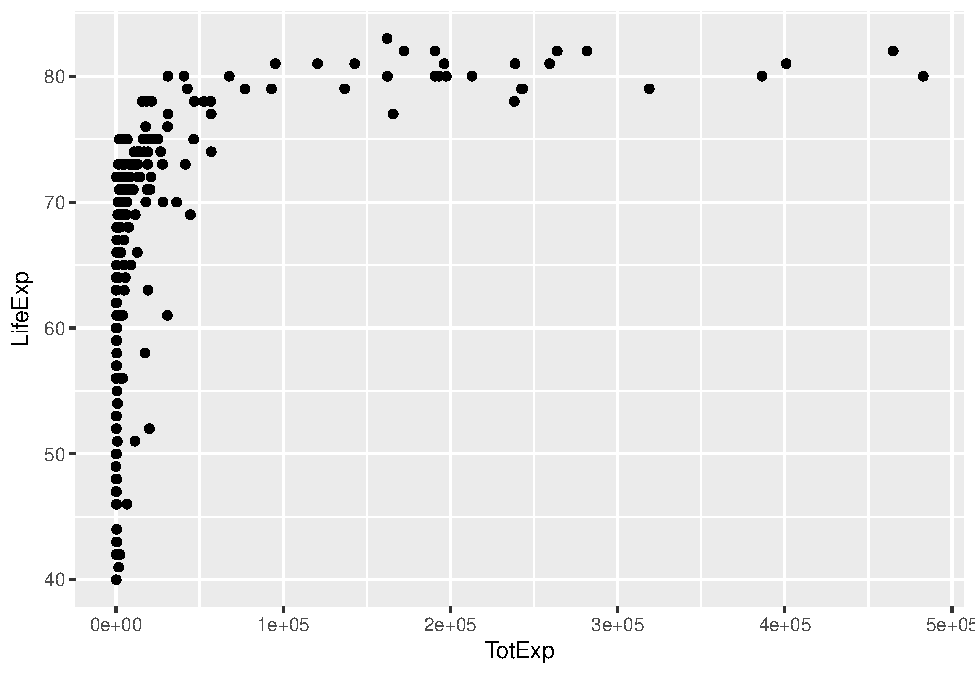
\includegraphics{JSturm_Assignment_12_files/figure-latex/scatterplot-lifexp-totexp-1.pdf}

\begin{verbatim}
## 
## Call:
## lm(formula = LifeExp ~ TotExp, data = who)
## 
## Residuals:
##     Min      1Q  Median      3Q     Max 
## -24.764  -4.778   3.154   7.116  13.292 
## 
## Coefficients:
##              Estimate Std. Error t value Pr(>|t|)    
## (Intercept) 6.475e+01  7.535e-01  85.933  < 2e-16 ***
## TotExp      6.297e-05  7.795e-06   8.079 7.71e-14 ***
## ---
## Signif. codes:  0 '***' 0.001 '**' 0.01 '*' 0.05 '.' 0.1 ' ' 1
## 
## Residual standard error: 9.371 on 188 degrees of freedom
## Multiple R-squared:  0.2577, Adjusted R-squared:  0.2537 
## F-statistic: 65.26 on 1 and 188 DF,  p-value: 7.714e-14
\end{verbatim}

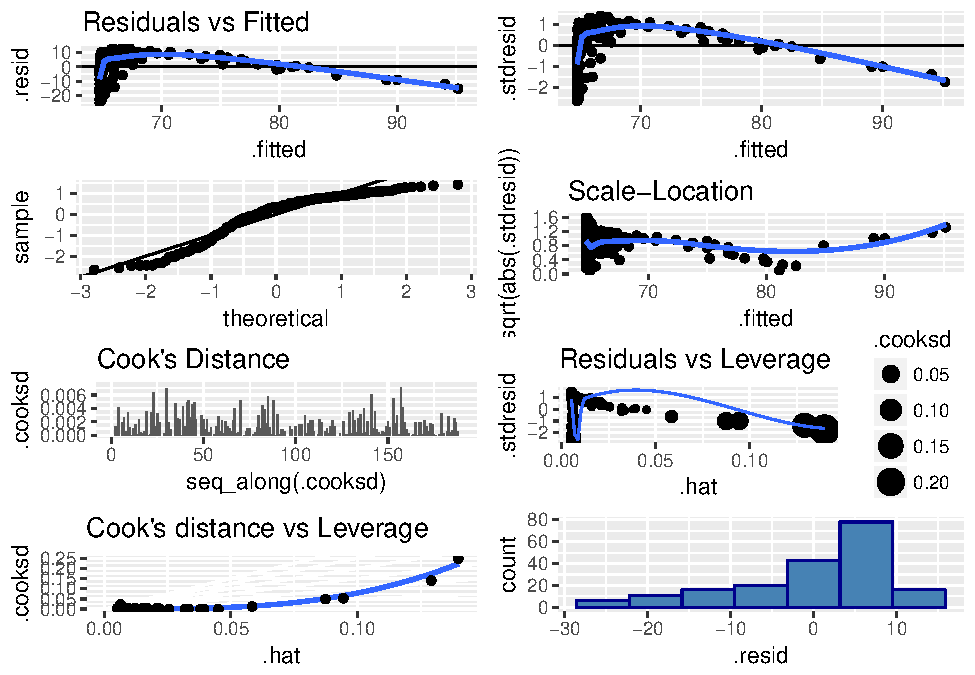
\includegraphics{JSturm_Assignment_12_files/figure-latex/simple-regression-1.pdf}

The F-statistic for this model is 65.2641982, and the p-value is
\(7.7139931\times 10^{-14}\). This tells us that the relationship
between the variables \texttt{LifeExp} and \texttt{TotExp} is likely not
due to chance.

With a low r-squared value of 0.2576922, the model is only able to
explain \(\approx 25\%\) of the variability. Furthermore, since the
residuals are not normally distributed, as can be seen in the plots,
this model is insufficient to explain the relationship between the data.

We can make use of the \texttt{gvlma} package to confirm our
interpretation.

\begin{verbatim}
## 
## Call:
## lm(formula = LifeExp ~ TotExp, data = who)
## 
## Coefficients:
## (Intercept)       TotExp  
##   6.475e+01    6.297e-05  
## 
## 
## ASSESSMENT OF THE LINEAR MODEL ASSUMPTIONS
## USING THE GLOBAL TEST ON 4 DEGREES-OF-FREEDOM:
## Level of Significance =  0.05 
## 
## Call:
##  gvlma(x = model1) 
## 
##                        Value   p-value                   Decision
## Global Stat        56.737011 1.405e-11 Assumptions NOT satisfied!
## Skewness           30.532757 3.283e-08 Assumptions NOT satisfied!
## Kurtosis            0.002804 9.578e-01    Assumptions acceptable.
## Link Function      26.074703 3.285e-07 Assumptions NOT satisfied!
## Heteroscedasticity  0.126747 7.218e-01    Assumptions acceptable.
\end{verbatim}

\section{2.}\label{section-1}

\begin{verbatim}
## 
## Call:
## lm(formula = m2.LifeExp ~ m2.TotExp)
## 
## Residuals:
##        Min         1Q     Median         3Q        Max 
## -308616089  -53978977   13697187   59139231  211951764 
## 
## Coefficients:
##               Estimate Std. Error t value Pr(>|t|)    
## (Intercept) -736527910   46817945  -15.73   <2e-16 ***
## m2.TotExp    620060216   27518940   22.53   <2e-16 ***
## ---
## Signif. codes:  0 '***' 0.001 '**' 0.01 '*' 0.05 '.' 0.1 ' ' 1
## 
## Residual standard error: 90490000 on 188 degrees of freedom
## Multiple R-squared:  0.7298, Adjusted R-squared:  0.7283 
## F-statistic: 507.7 on 1 and 188 DF,  p-value: < 2.2e-16
\end{verbatim}

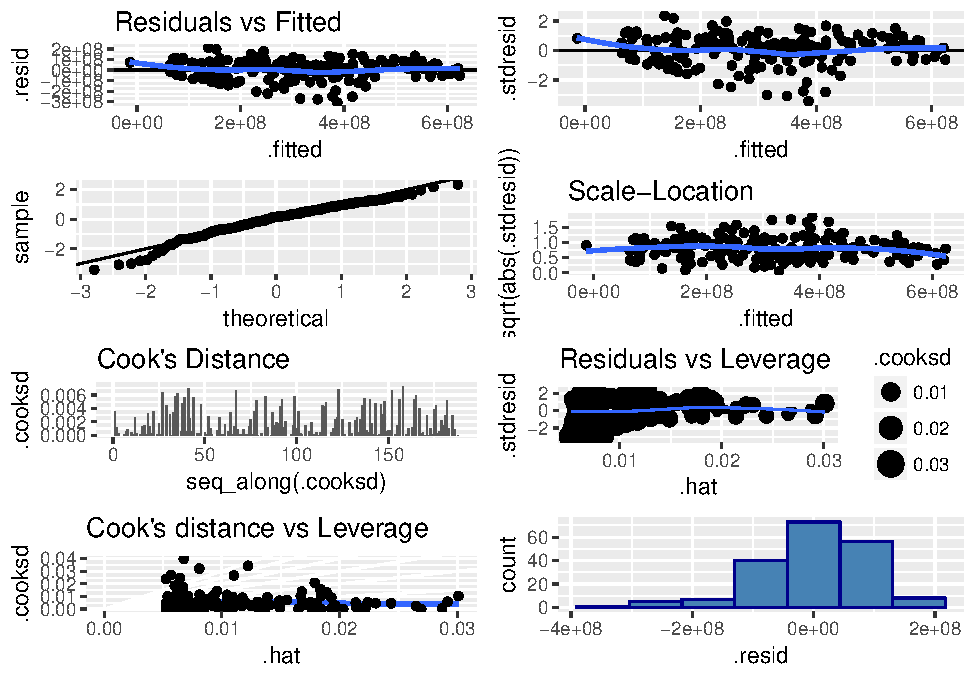
\includegraphics{JSturm_Assignment_12_files/figure-latex/model-two-1.pdf}

\begin{verbatim}
## 
## Call:
## lm(formula = m2.LifeExp ~ m2.TotExp)
## 
## Coefficients:
## (Intercept)    m2.TotExp  
##  -736527909    620060216  
## 
## 
## ASSESSMENT OF THE LINEAR MODEL ASSUMPTIONS
## USING THE GLOBAL TEST ON 4 DEGREES-OF-FREEDOM:
## Level of Significance =  0.05 
## 
## Call:
##  gvlma(x = model2) 
## 
##                      Value   p-value                   Decision
## Global Stat        27.8117 1.362e-05 Assumptions NOT satisfied!
## Skewness           17.1372 3.478e-05 Assumptions NOT satisfied!
## Kurtosis            7.4581 6.315e-03 Assumptions NOT satisfied!
## Link Function       2.9866 8.396e-02    Assumptions acceptable.
## Heteroscedasticity  0.2299 6.316e-01    Assumptions acceptable.
\end{verbatim}

Other than the higher standard error of 90492392, this model performs
considerably better than the original one. It has an f-statistic of
507.6967054 and a p-value of \(0\). It has a much higher r-squared value
of 0.7297673, which tells us that it's significantly better at
explaining the variability in the data. From the summary plots, the
residuals appear more normal, and randomly distributed, than in the
first model.

In summary, this model outperforms the first by most measures, but still
fails most assumptions needed for linear regression.

\section{3.}\label{section-2}

\subsection{3.1}\label{section-3}

The equation from model 2 is \(y^{4.6} =\) -736527909 +
620060215\(\cdot x^{0.06}\).

\(y^{4.6} =\) -736527909 + 620060215 \(\cdot (1.5) \ \to\) 193562413

\(y = \text{LifeExp} = \sqrt[4.6]{193562414} \approx\) 63.3115334

\subsection{3.2}\label{section-4}

\(y^{4.6} =\) -736527909 + 620060215 \(\cdot (2.5) \ \to\) 813622629

\(y = \text{LifeExp} = \sqrt[4.6]{813622629} \approx\) 86.5064485

\section{4.}\label{section-5}

We want to build the model LifeExp = b0+b1 x PropMd + b2 x TotExp +b3 x
PropMD x TotExp.

\begin{verbatim}
## 
## Call:
## lm(formula = LifeExp ~ PropMD + TotExp + PropMD * TotExp, data = who)
## 
## Residuals:
##     Min      1Q  Median      3Q     Max 
## -27.320  -4.132   2.098   6.540  13.074 
## 
## Coefficients:
##                 Estimate Std. Error t value Pr(>|t|)    
## (Intercept)    6.277e+01  7.956e-01  78.899  < 2e-16 ***
## PropMD         1.497e+03  2.788e+02   5.371 2.32e-07 ***
## TotExp         7.233e-05  8.982e-06   8.053 9.39e-14 ***
## PropMD:TotExp -6.026e-03  1.472e-03  -4.093 6.35e-05 ***
## ---
## Signif. codes:  0 '***' 0.001 '**' 0.01 '*' 0.05 '.' 0.1 ' ' 1
## 
## Residual standard error: 8.765 on 186 degrees of freedom
## Multiple R-squared:  0.3574, Adjusted R-squared:  0.3471 
## F-statistic: 34.49 on 3 and 186 DF,  p-value: < 2.2e-16
\end{verbatim}

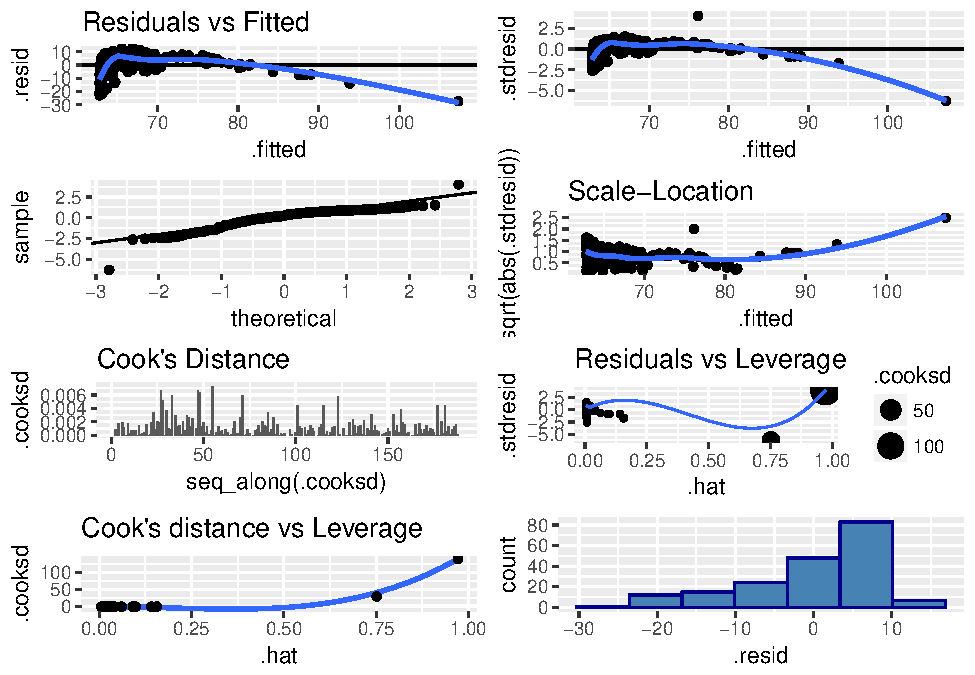
\includegraphics{JSturm_Assignment_12_files/figure-latex/model-three-1.pdf}

\begin{verbatim}
## 
## Call:
## lm(formula = LifeExp ~ PropMD + TotExp + PropMD * TotExp, data = who)
## 
## Coefficients:
##   (Intercept)         PropMD         TotExp  PropMD:TotExp  
##     6.277e+01      1.497e+03      7.233e-05     -6.026e-03  
## 
## 
## ASSESSMENT OF THE LINEAR MODEL ASSUMPTIONS
## USING THE GLOBAL TEST ON 4 DEGREES-OF-FREEDOM:
## Level of Significance =  0.05 
## 
## Call:
##  gvlma(x = model3) 
## 
##                      Value   p-value                   Decision
## Global Stat        87.0703 0.000e+00 Assumptions NOT satisfied!
## Skewness           33.4219 7.418e-09 Assumptions NOT satisfied!
## Kurtosis            0.5600 4.543e-01    Assumptions acceptable.
## Link Function      52.7284 3.830e-13 Assumptions NOT satisfied!
## Heteroscedasticity  0.3599 5.486e-01    Assumptions acceptable.
\end{verbatim}

The F-statistic for this model is 34.4883268, and the p-value is \(0\).
With a low r-squared value of 0.2576922, the model is only able to
explain \(\approx 35\%\) of the variability. There are a few outliers in
this model, which introduces a lot of skew in the residual plots, making
them not normally distributed. Overall, this model fared similarly to
the first, and worse than the second.

\section{5.}\label{section-6}

PropMD = 0.03, TotExp = 14.

Using model 3:

LifeExp = 62.7727033 + 1497.4939525\(\cdot (0.03)\) +
10\^{}\{-4\}\(\cdot (14)\) -0.0060257\(\cdot (0.03 \cdot 14)\)

LifeExp \(\approx\) 107.7010653.

This prediction does not seem realistic, since the total personal and
government expenditure is near the minimum, yet life expentancy exceeds
that of any country in the dataset.


\end{document}
